\documentclass[12pt,letterpaper]{article}


\newcommand{\doctitle}{Scientific Computing Homework 2}
\newcommand{\docauthor}{Matthew Duschenes}
\newcommand{\docaffil}{Department of Applied Physics, University of Michigan}
\newcommand{\docheader}{NERS 570 \ - Homework 2 - \docauthor}
\newcommand{\docfooter}{\docaffil}


% Margins
\usepackage[margin=0.75in,marginparsep=0pt,paperwidth=216mm,paperheight=279mm]{geometry}

% Headers
\usepackage{fancyhdr}
\geometry{headheight=15pt}
\renewcommand{\headrulewidth}{0.4pt}% default is 0.4pt
\renewcommand{\footrulewidth}{0.4pt}% default is 0pt
\geometry{headheight=15pt}
\geometry{headsep=10pt}
\setlength{\skip\footins}{10pt} % gap between text and footer
\fancyhf{}
\fancyhead[R]{\docheader}
\fancyfoot[LE,RO]{\thepage}
\fancyfoot[LO,RE]{\docfooter}

% \makeatletter
% \if@twoside
% \fancyfoot[LE,RO]{\thepage}
% \fancyfoot[LO,RE]{\docfooter}
% \else
% \fancyfoot[R]{\thepage}
% \fancyfoot[L]{\docfooter}
% \fi
% \makeatother
% \fancyhead[R]{\docheader}


% Title
\usepackage{titling}
% \usepackage[affil-it]{authblk}
\usepackage[nodayofweek]{datetime}
\usepackage[super]{nth}

% \newdateformat{monthdayyear}{%
%   \monthname[\THEMONTH]~\THEDAY,~ \THEYEAR}
% \newdateformat{mydate}{\monthname[\THEMONTH] \nth[\THEDAY], \THEYEAR}


% Make Title
\pagestyle{fancy}
% \renewcommand*{\Authfont}{\bfseries}
% \renewcommand*{\Affilfont}{\normalfont\itshape}
\pretitle{\begin{center}\vskip -50pt}%
\title{\large \doctitle}
\posttitle{\end{center}}
\preauthor{\begin{center} \vskip -20pt}
\author{}
\postauthor{\end{center} \vskip -20pt}
\predate{\begin{center} \vskip -20pt}
\date{}%\small{\today}}
\postdate{\end{center} \vskip -20pt}% -42.5pt


% Fonts
\usepackage[singlespacing]{setspace}

 
% Math
\usepackage{amsmath}
\usepackage{amssymb}
\usepackage{physics}




 % Commands
\newcommand{\reals}{\mathbb{R}}
\DeclareMathOperator*{\argmax}{arg\,max}
\DeclareMathOperator*{\argmin}{arg\,min}





%%%%%%%%%%%%%%%%%%%%%%%%%%%%%%%%%%%%%%%%%%%%%%%%%%%
\begin{document}
\maketitle
\thispagestyle{fancy}
\singlespacing
%%%%%%%%%%%%%%%%%%%%%%%%%%%%%%%%%%%%%%%%%%%%%%%%

\section{Spectral Radius of Fixed Point Methods}
Fixed Point iterative methods involve finding the solutions to 
\begin{equation}
  Ax = b  
\end{equation}
by decomposing the matrix into a form such that iterations are
\begin{equation}
  x_{n+1} = Bx_{n} + c,  
\end{equation}
where $B$ is matrix that is typically a function of $A$, and $c$ is a function of $A$ and $b$. These iteration matrices are generally most easily expressed when $A$ is decomposed as its diagonal, lower, and upper triangular components:
\begin{equation}
  A = D + L + U,
\end{equation} 
since the forms of these matrices make them easily invertible for use in the iterative updates to $x$.

Given an initial guess $x_0$ the error $e_{n} = x_{n} - x$ is
\begin{equation}
  e_n = B^{n}e_0, 
\end{equation}
and the relative norm of the error is:
\begin{equation}
  \frac{\norm{e_{n}}}{\norm{e_{0}}} \leq \norm{B^n}.
\end{equation} 

This norm of $\norm{B^n}$ can be approximated by upper bounds, and in the case of the 2-norm, in terms of the spectral radius $\rho(B)$:
\begin{equation}
  \norm{B^n} \leq \norm{B}^n \leq \rho(B)^n.
\end{equation}
Therefore the spectral radius of $B$ can be found from either directly calculating (through some other iterative method using a numerical library) for the eigenvalues of $B$, or from measuring the norms of the residual over the iterations, with the last iteration likely giving the best estimate for the spectral radius:

\begin{equation}
  \rho(B) = \max_{\lambda} \abs{\lambda(B)} = {\left(\frac{\norm{e_{n}}}{\norm{e_{0}}}\right)}^{1/n}.
\end{equation}



\subsection{Jacobi Method}
For the Jacobi method, the iterations proceed such that
\begin{align}
  B &= -D^{-1}(L+U) \\
  c &= D^{-1}b.
\end{align}



\subsection{Gauss-Seidel Method}
For the Gauss-Seidel method, the iterations proceed such that
\begin{align}
  B &= -(D+L)^{-1}U \\
  c &= (D+L)^{-1}b.
\end{align}


\subsection{Fixed Point Iteration Results}
As shown in Figure \ref{fig:FixedPt}, the numerical and analytic 


\begin{figure}[ht]
  \centering
  %  trim={<left> <lower> <right> <upper>}
  % \captionsetup{skip=-12pt,format=hang}
  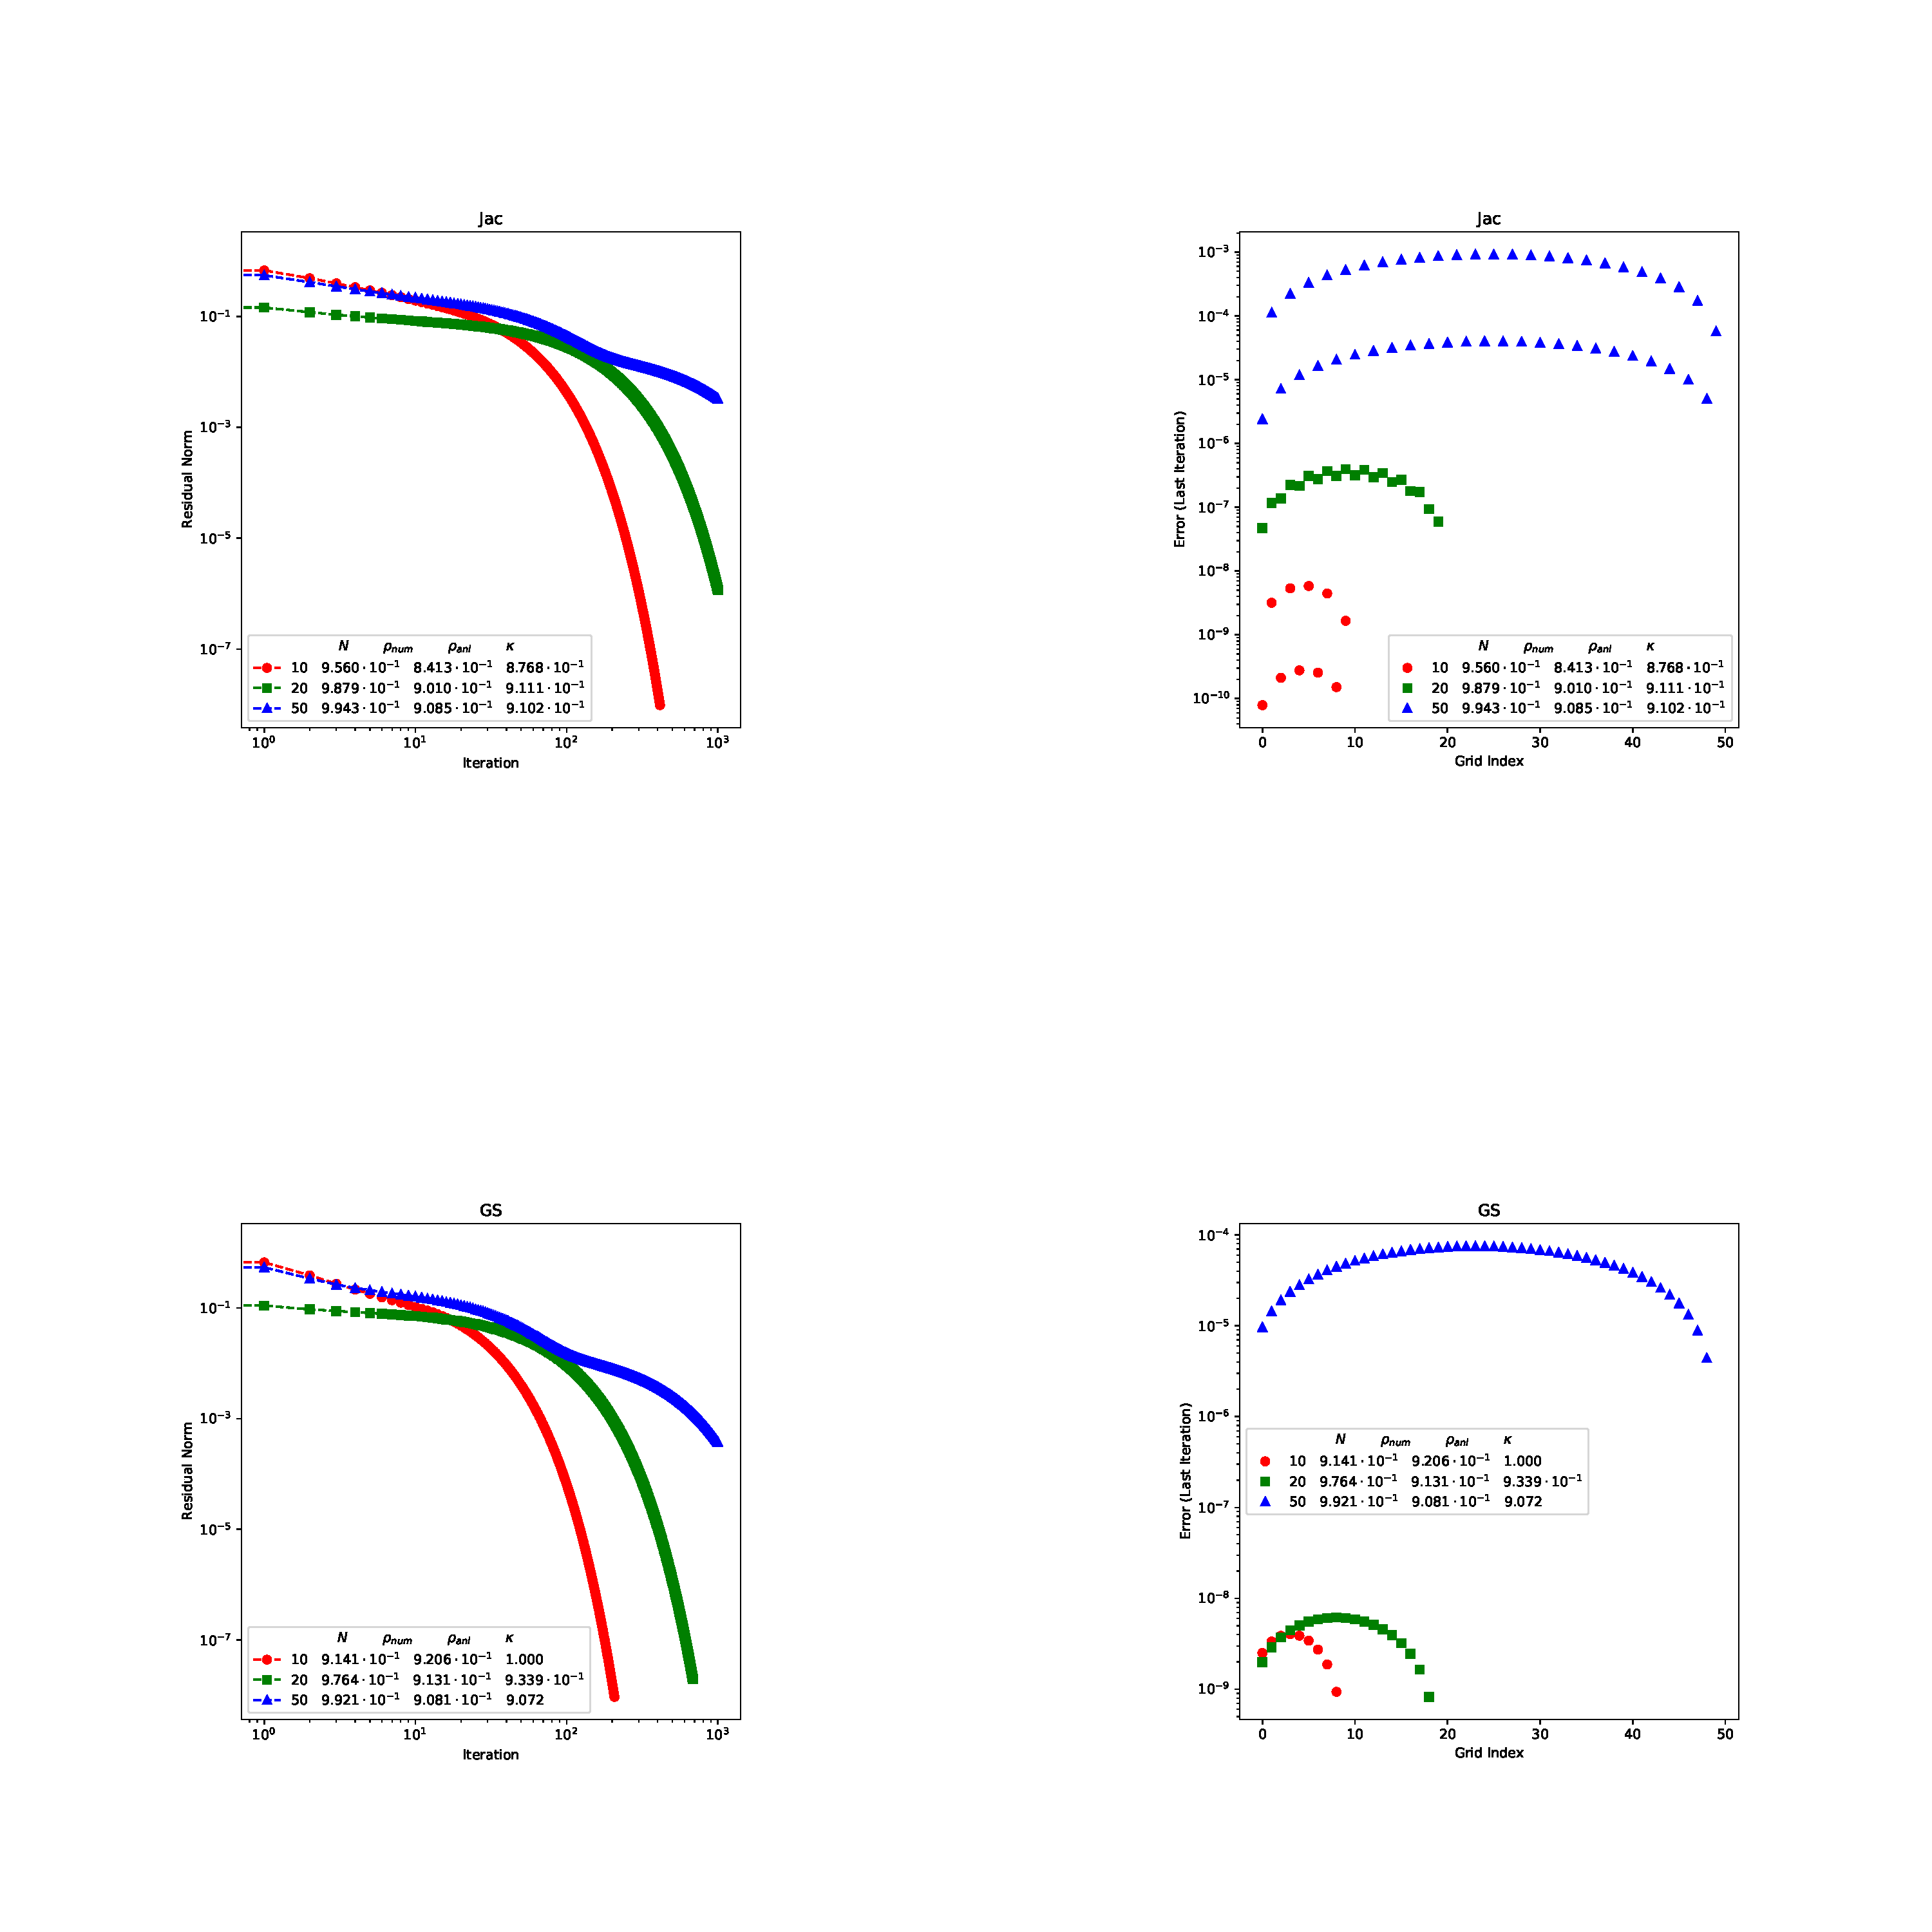
\includegraphics[width=0.6\textwidth,trim={0 0 0 6cm},clip]{Ex1.pdf}
  % \vspace{-8pt}
  \caption{Residual norms over iterations, and final solution error for $d=1$ Laplace's equation, using Jacobi and Gauss-Seidel methods. Shown in the legend are eigenvalue statistics for various grid sizes.}
  \label{fig:FixedPt}
\end{figure}

%%%%%%%%%%%%%%%%%%%%%%%%%%%%%%%%%%%%%%%%%%%%%%%%
% \newpage
% \bibliographystyle{unsrt}
% \bibliography{mduschen_Ex1.bib}

\end{document}